\begin{name}
	{\tenchude}
	{TOÁN 11}
	{LỚP TOÁN THẦY PHÁT}
	{Thời gian: 15 phút - Không kể thời gian phát đề}
\end{name}
\Opensolutionfile{ans}[ans/ans-1-B2-1]
\caulc {\textbf{\textit{(3,0 điểm)}}} %\subsubsection{Câu trắc nghiệm nhiều phương án lựa chọn}
% Học sinh trả lời từ câu $1$ đến câu $12$. Mỗi câu hỏi học sinh chỉ chọn một phương án.
%%==========Câu 1
\begin{ex}%[1D1N3-1] 
Trong các công thức sau, công thức nào đúng?
\choice
{$\cos (a-b)=\cos a\sin b+\sin a\cos b$}
{\True $\sin (a-b) = \sin a\cos b - \cos a\sin b$}
{$\sin (a+b) = \sin a\cos b - \cos a\sin b$}
{$\cos (a+b)=\cos a\cos b+\sin a\sin b$}
\loigiai{
	Công thức đúng: $\sin (a-b)=\sin a\cos b-\cos a\sin b$.
}
\end{ex}

%%==========Câu 2
\begin{ex}%[1D1N3-2]
Đẳng thức nào sau đây là đúng?
\choice
{$\cos \left(\alpha +\dfrac{\pi }{6}\right)=\dfrac{1}{2}\cos \alpha +\dfrac{\sqrt{3}}{2}\sin \alpha $}
{$\cos \left(\alpha +\dfrac{\pi }{6}\right)=\dfrac{1}{2}\sin \alpha -\dfrac{\sqrt{3}}{2}\cos \alpha $}
{$\cos \left(\alpha +\dfrac{\pi }{6}\right)=\dfrac{\sqrt{3}}{2}\cos \alpha +\dfrac{1}{2}\sin \alpha $}
{\True $\cos \left(\alpha +\dfrac{\pi }{6}\right)=\dfrac{\sqrt{3}}{2}\cos \alpha -\dfrac{1}{2}\sin \alpha $}
\loigiai{
	Ta có: $\cos \left(\alpha +\dfrac{\pi }{6}\right)=\cos \alpha \cos \dfrac{\pi }{6}-\sin \alpha \sin \dfrac{\pi }{6}=\dfrac{\sqrt{3}}{2}\cos \alpha -\dfrac{1}{2}\sin \alpha$.}
\end{ex}

%%==========Câu 3
\begin{ex}%[1D1N3-3]
Trong các công thức sau, công thức nào \textbf{sai}?
\choice
{$\cos 2a={\cos ^2}a-{\sin ^2}a$}
{\True $\sin 2a={\cos ^2}a-{\sin ^2}a$}
{$\cos 2a = 2{\cos ^2}a-1$}
{$\sin 2a=2\sin a\cos a$}
\loigiai{
	Ta có: $\sin 2a=2\sin a\cos a$ nên $\sin 2a={\cos ^2}a-{\sin ^2}a$ sai.}
\end{ex}

%%==========Câu 4
\begin{ex}%[1D1N3-1]
Trong các công thức sau, công thức nào đúng?
\choice
{$\tan (a-b) = \dfrac{\tan a + \tan b}{1 - \tan a\tan b}$}
{$\tan (a-b)=\tan a\tan b-\cot a\cot b$}
{\True $\tan (a+b) = \dfrac{\tan a + \tan b}{1 - \tan a\tan b}$}
{$\tan (a+b)=\tan a\cot a+\tan b\cot a$}
\loigiai{
	Ta có: $\tan (a-b)=\dfrac{\tan a-\tan b}{1+\tan a\tan b}$ và $\tan (a+b) = \dfrac{\tan a + \tan b}{1 - \tan a\tan b}$.}
\end{ex}

%%==========Câu 6
\begin{ex}%[1D1N3-1]
Trong các công thức sau, công thức nào \textbf{sai}?
\choice
{$\sin x+\sin y=2\sin \dfrac{x+y}{2}\cos \dfrac{x-y}{2}$}
{$\sin x-\sin y=2\cos \dfrac{x+y}{2}\sin \dfrac{x-y}{2}$}
{$\cos x+\cos y=2\cos \dfrac{x+y}{2}\cos \dfrac{x-y}{2}$}
{\True $\cos x-\cos y=2\sin \dfrac{x+y}{2}\sin \dfrac{x-y}{2}$}
\loigiai{
	Ta có: $\cos x-\cos y=-2\sin \dfrac{x+y}{2}\sin \dfrac{x-y}{2}$ nên $\cos x-\cos y=2\sin \dfrac{x+y}{2}\sin \dfrac{x-y}{2}$ sai.}
\end{ex}

%%==========Câu 7
% \begin{ex}%[1D1N3-2]
% Tính giá trị của biểu thức $A=\tan \left(x-\dfrac{3\pi }{4}\right)$ biết $\tan x=3$.
% \choice
% {$2$}
% {$-\dfrac{1}{2}$}
% {$\dfrac{1}{2}$}
% {\True $-2$}
% \loigiai{
% 	Ta có: $A=\tan \left(x-\dfrac{3\pi }{4}\right)=\dfrac{\tan x-\tan \dfrac{3\pi }{4}}{1+\tan x\cdot\tan \dfrac{3\pi }{4}}=\dfrac{3-(-1)}{1+3\cdot(-1)}=-2$.}
% \end{ex}
\begin{ex}%[Huỳnh Đức Vũ, dự án giảng K10-11]%[1D1N3-4]
Mệnh đề nào sau đây \textbf{sai}.
\choice
{\True $\cos a \sin b=\dfrac{1}{2}[\sin (a-b)-\sin (a+b)]$}
{$\sin a \cos b=\dfrac{1}{2}[\sin (a-b)+\sin (a+b)]$}
{$\cos a \cos b=\dfrac{1}{2}[\cos (a-b)+\cos (a+b)]$}
{$\sin a \sin b=\dfrac{1}{2}[\cos (a-b)-\cos (a+b)]$}
\loigiai
{Công thức sai là $\cos a \sin b=\dfrac{1}{2}[\sin (a-b)-\sin (a+b)]$.}
\end{ex}
% %%==========Câu 8
% \begin{ex}%[1D1H3-3]
% Tính giá trị của biểu thức $P=(1-2\cos 2a)(1+3\cos 2a)$ biết $\sin a=\dfrac{1}{3}$.
% \choice
% {\True $-\dfrac{50}{27}$}
% {$-\dfrac{92}{27}$}
% {$1$}
% {$-\dfrac{5}{3}$}
% \loigiai{
% 	Ta có: $\cos 2a=1-2{\sin ^2}a=1-2\cdot{{\left(\dfrac{1}{3}\right)}^2}=\dfrac{7}{9}$.\\
% 	Suy ra $P=\left(1-2\cdot\dfrac{7}{9}\right)\left(1+3\cdot\dfrac{7}{9}\right)=-\dfrac{50}{27}$.}
% \end{ex}

% %%==========Câu 9
% \begin{ex}%[1D1H3-4]
% Cho $\cos 2\alpha =\dfrac{3}{5}$. Tính giá trị của biểu thức $P = \cos \alpha\cos 3\alpha$.
% \choice
% {$-\dfrac{9}{25}$}
% {$-\dfrac{4}{25}$}
% {\True $\dfrac{4}{25}$}
% {$\dfrac{9}{25}$}
% \loigiai{
% 	Ta có: $\cos x\cos y=\dfrac{1}{2}\left[ \cos \left(x+y\right)+\cos \left(x-y\right) \right]$.\\
% 	Suy ra 
% 	$ \begin{aligned}[t] 
% 		P&=\cos \alpha \cdot\cos 3\alpha =\dfrac{1}{2}\left(\cos 4\alpha +\cos (-2\alpha)\right)=\dfrac{1}{2}(\cos 4\alpha +\cos 2\alpha) \\
% 		&=\dfrac{1}{2}(2{\cos ^2}2\alpha -1+\cos 2\alpha)=\dfrac{1}{2}\left(2\cdot\dfrac{9}{25}-1+\dfrac{3}{5}\right)=\dfrac{4}{25}.
% 	\end{aligned}$}
% \end{ex}


%%==========Câu 11



\Closesolutionfile{ans}
% \indapan{9}{ans/ans-1-B2-1}

\cauds{\textbf{\textit{(2,0 điểm)}}}
% Học sinh trả lời từ câu $1$ đến câu $4$. Trong mỗi ý a), b), c), d) ở mỗi câu, học sinh chọn \textbf{đúng} hoặc \textbf{sai}.
\Opensolutionfile{ans}[ans/ans-BOTCVII-2]
%%==========Câu 1
\begin{ex}%[1D1N2-2]
	Cho biết $\tan x=\sqrt{2}$ và $0<x<90^\circ$. Khi đó:
	\choiceTF
	{\True $\cos x>0$}
	{\True $\cos x=\dfrac{\sqrt{3}}{3}$}
	{\True $\sin x=\dfrac{\sqrt{6}}{3}$}
	{$\cos (x-30^\circ)=\dfrac{3-\sqrt{6}}{6}$}
	\loigiai{
	Vì $0<x<90^{\circ}$ nên $\cos x>0$.\\
	Ta có: $\dfrac{1}{\cos ^2 x}=1+\tan ^2 x=1+2=3 \Rightarrow \cos ^2 x=\dfrac{1}{3} \Rightarrow \cos x=\dfrac{\sqrt{3}}{3}$.\\
	Mặt khác: $\tan x=\dfrac{\sin x}{\cos x} \Rightarrow \sin x=\tan x \cos x=\dfrac{\sqrt{6}}{3}$.\\
	$\cos (x-30^\circ)=\cos x\cos 30^\circ+\sin x\sin 30^\circ\dfrac{\sqrt{3}}{3}\cdot \dfrac{\sqrt{3}}{2}+\dfrac{\sqrt{6}}{3}\cdot \dfrac{1}{2}=\dfrac{3+\sqrt{6}}{6}$.
}
\end{ex}

%%==========Câu 2
\begin{ex}%[1D1H3-2]
	Biết $\sin a=\dfrac{8}{17}$, $\tan b=\dfrac{5}{12}$ và $a$, $b$ là các góc nhọn. Khi đó:
	\choiceTF
	{\True $\tan a=\dfrac{8}{15}$}
	{\True $\sin (a-b)=\dfrac{21}{221}$}
	{$\cos (a+b)=\dfrac{14}{22}$}
	{$\tan (a+b)=\dfrac{17}{14}$}
	\loigiai{
	Vì $a$, $b$ là các góc nhọn nên $\cos a>0$, $\cos b>0$.\\
	Ta có: $\cos a=\sqrt{1-\sin ^2 a}=\dfrac{15}{17} \Rightarrow \tan a=\dfrac{\sin a}{\cos a}=\dfrac{8}{15}$;\\
	$\cos b=\sqrt{\dfrac{1}{1+\tan ^2 b}}=\dfrac{12}{13} \Rightarrow \sin b=\cos b \tan b=\dfrac{5}{13}$.\\
	Khi đó: $\sin (a-b)=\sin a \cos b-\cos a \sin b=\dfrac{8}{17} \cdot \dfrac{12}{13}-\dfrac{15}{17} \cdot \dfrac{5}{13}=\dfrac{21}{221}$.\\
	$\cos (a+b)=\cos a \cos b-\sin a \sin b=\dfrac{15}{17} \cdot \dfrac{12}{13}-\dfrac{8}{17} \cdot \dfrac{5}{13}=\dfrac{140}{221}$.\\
	$\tan (a+b)=\dfrac{\tan a+\tan b}{1-\tan a \tan b}=\dfrac{\dfrac{8}{15}+\dfrac{5}{12}}{1-\dfrac{8}{15} \cdot \dfrac{5}{12}}=\dfrac{171}{140}$.
}
\end{ex}

% %%==========Câu 3
% \begin{ex}%[1D1H3-2]
% 	Biết $0<a, b<\dfrac{\pi}{2}$, $a+b=\dfrac{\pi}{4}$ và $\tan a \tan b=3-2 \sqrt{2}$. Khi đó:
% 	\choiceTF
% 	{\True $\tan a+\tan b=-2+2\sqrt{2}$}
% 	{\True $\tan a=-1+\sqrt{2}$}
% 	{$\tan b=-1-\sqrt{2}$}
% 	{$\tan a-\tan b=-2-2\sqrt{2}$}
% 	\loigiai{
% 	$\tan (a+b)=\dfrac{\tan a+\tan b}{1-\tan a \tan b} \Rightarrow \tan a+\tan b=\tan (a+b)(1-\tan a \tan b)$.\\
% 	Mà $a+b=\dfrac{\pi}{4}$ và $\tan a \tan b=3-2 \sqrt{2} \Rightarrow \tan a+\tan b=\tan \dfrac{\pi}{4}[1-(3-2 \sqrt{2})]=-2+2 \sqrt{2}$.\\
% 	Đặt $S=\tan a+\tan b$; $P=\tan a \tan b$.\\
% 	Khi đó $\tan a$, $\tan b$ là nghiệm của phương trình
% 	\[X^2-S X+P=0 \Leftrightarrow X^2-(2 \sqrt{2}-2) X+3-2 \sqrt{2}=0 \Leftrightarrow X=-1+\sqrt{2}.\]
% 	Suy ra $\tan a=\tan b=-1+\sqrt{2}$.
% }
% \end{ex}

% %%==========Câu 4
% \begin{ex}%[1D1H3-3]
% 	Biết $\tan \alpha=2$. Khi đó:
% 	\choiceTF
% 	{$\cot \alpha =-\dfrac{1}{2}$}
% 	{\True $\cos 2\alpha =-\dfrac{3}{5}$}
% 	{\True $\sin 2\alpha =\dfrac{4}{5}$}
% 	{\True $\tan 2\alpha =-\dfrac{4}{3}$}
% 	\loigiai{
% 	Ta có: $\cos 2 \alpha=2 \cos ^2 \alpha-1=\dfrac{2}{\tan ^2 \alpha+1}-1=\dfrac{2}{5}-1=-\dfrac{3}{5}$;\\
% 	$\sin 2 \alpha=2 \sin \alpha \cos \alpha=2 \tan \alpha \cos ^2 \alpha=\dfrac{2 \tan \alpha}{\tan ^2 \alpha+1}=\dfrac{4}{5}$;\\
% 	$\tan 2 \alpha=\dfrac{\sin 2 \alpha}{\cos 2 \alpha}=-\dfrac{4}{3}$.
% }
% \end{ex}

\Closesolutionfile{ans}
% \indapan{3}{ans/ans-BOTCVII-2}

% \newpage
\caukq{\textbf{\textit{(3,0 điểm)}}} %\subsubsection{Câu trắc nghiệm trả lời ngắn}
% Học sinh trả lời từ câu $1$ đến câu $6$.
\Opensolutionfile{ans}[ans/ans-1-B2-3]
\begin{ex}%[1D1H3-4]
Biết $\cos a=\dfrac{1}{3}$, $\sin b=\dfrac{3}{5}$, giá trị của biểu thức $\cos (a + b)\cos (a - b)$ bằng phân số tối giản $\dfrac{m}{n}$. Tính $m+n$.
% \choice
% {$-\dfrac{238}{225}$}
% {$\dfrac{238}{225}$}
% {\True $-\dfrac{56}{225}$}
% {$-\dfrac{112}{225}$}
\shortans{169}
\loigiai{
	Ta có: 
	$ \begin{aligned}[t] 
		\cos (a+b)\cos (a-b)&=\dfrac{1}{2}\left[ \cos \left(a+b+a-b\right)+\cos \left((a+b)-(a-b)\right) \right] \\
		&= \dfrac{1}{2}\left(\cos 2a+\cos 2b\right)=\dfrac{1}{2}\left(2{\cos ^2}a-1+1-2{\sin ^2}b\right)\\
		&= \dfrac{1}{2}\left(2\cdot\dfrac{1}{9}-2\cdot\dfrac{9}{25}\right)=-\dfrac{56}{225}.
	\end{aligned}$
}
\end{ex}
% %%==========Câu 13
% \begin{ex}%[1D1N2-2]
% Tính $\cot \dfrac{3\pi }{11}$, ta được kết quả (làm tròn đến một chữ số thập phân).
% \shortans{$0{,}9$}
% \loigiai{
% 	\begin{itemize}
% 		\item Dùng máy tính CASIO fx 580VN.
% 		\item Chuyển đơn vị Radian: \shiftk \menuk \twok \twok.
% 		\item Tính $\cot \dfrac{3\pi }{11}$: bấm $\dfrac{1}{\tan \dfrac{3\pi }{11}}\approx 0{,}8665\approx 0{,}9$.
% 	\end{itemize}
% }
% \end{ex}

% %%==========Câu 14
% \begin{ex}%[1D1H3-2]
% \immini{
% Cho tam giác $ABC$ vuông tại $B$ và có hai cạnh góc vuông là $AB=5$, $BC=3$. Vẽ điểm $D$ nằm trên tia đối của tia $CB$ thỏa mãn $\widehat{CAD}=45^\circ $. Tính độ dài cạnh $CD$ (xem hình minh họa).
% }{
% \begin{tikzpicture}[scale=.8,font=\footnotesize]
% 	\path (0,0) coordinate (B) (0,3) coordinate (A) (1.5,0) coordinate (C) (6,0) coordinate (D);
% 	\draw (C)--(A)--node[left]{$5$}(B)--node[below]{$3$}(C)--(D)--(A);
% 	\draw pic["$45^\circ$"{scale=.7},draw, angle radius = 12pt,angle eccentricity=1.6]{angle = C--A--D};
% 	\foreach \i/\j/\k in {A/B/D}{
% 		\draw[cyan] ($(\j)!7pt!(\i)$)--($(\j)!7pt!(\k)-(\j)+(\j)!7pt!(\i)$)--($(\j)!7pt!(\k)$);};
% 	\foreach \i/\j in {A/100,B/-135,C/-90,D/-45}
% 	\fill (\i) circle (1.2pt) node[shift={(\j:2.5mm)}]{$\i$};
% \end{tikzpicture}
% }

% \shortans{$17$}
% \loigiai{
% 	Xét tam giác $ABC$ vuông tại $B$ có: $\tan\widehat{BAC}=\dfrac{3}{5}$.\\
% 	Ta lại có: $\widehat{BAD}=\widehat{BAC}+\widehat{CAD}$, suy ra:\\
% 	$ \begin{aligned}[t] 
% 		\tan\widehat{BAD}&=\tan\left(\widehat{BAC}+\widehat{CAD}\right)=\tan\left(\widehat{BAC}+45^\circ \right) \\
% 		&= \dfrac{\tan\widehat{BAC}+\tan 45^\circ}{1-\tan\widehat{BAC}\cdot \tan45^\circ }=\dfrac{\dfrac{3}{5}+1}{1-\dfrac{3}{5}\cdot 1}=4.
% 	\end{aligned}$\\
% 	Xét tam giác $ABD$ vuông tại $B$ có	$\tan\widehat{BAD}=\dfrac{BD}{AB}\Rightarrow BD=\tan\widehat{BAD}\cdot AB=4\cdot 5=20$.\\
% 	Suy ra $CD=BD-BC=20-3=17$.}
% \end{ex}
\begin{ex}%[1D1H3-3]
Cho $\sin a-\cos a=\dfrac{1}{5}\;(90^\circ<a<270^\circ)$. Tính giá trị của biểu thức $\tan 2a$ (làm tròn đến một chữ số thập phân).
\shortans{$3{,}4$}
\loigiai{
	Ta có: $\sin a-\cos a=\dfrac{1}{5}\Leftrightarrow \sin a=\cos a+\dfrac{1}{5}$.\\
	Mặt khác: ${\sin ^2}a+{\cos ^2}a=1$.\\
	Thay vào ta có: $\left(\cos a+\dfrac{1}{5}\right)^2+{\cos^2} a=1\Leftrightarrow 2{\cos ^2}a+\dfrac{2}{5}\cos a-\dfrac{24}{25}=0\Leftrightarrow \left[ \begin{matrix}
		\cos a=\dfrac{-4}{5} \\
		\cos a=\dfrac{3}{5}.\\
	\end{matrix} \right.$\\
	Vì $90^\circ<a<270^\circ\Rightarrow \cos a<0$. Do đó $\cos a=-\dfrac{4}{5}$.\\
	Nên $\sin a=\cos a+\dfrac{1}{5}=-\dfrac{3}{5}\Rightarrow \tan a=\dfrac{\sin a}{\cos a}=\dfrac{3}{4}\Rightarrow \tan 2a=\dfrac{2\tan a}{1-{\tan ^2}a}=\dfrac{24}{7}$.\\
	Suy ra $\tan 2a\approx 3{,}4$.}
\end{ex}
%%==========Câu 15
\begin{ex}%[1D1V3-7]
Đèo Hải Vân là ranh giới tự nhiên của thành phố Đà Nẵng và tỉnh Thừa Thiên-Huế. Hầm được khởi công ngày $27/8/2000$ và khánh thành ngày $5/6/2005$. Đây là hầm đường bộ dài nhất, hiện đại nhất Đông Nam Á và là một trong $30$ đường hầm dài nhất trên thế giới. Trong kiến trúc, có hình nửa đường tròn để có thể chịu lực tốt. Trong hình bên, cổng Đèo Hải Vân được ghép bởi sáu cung vật liệu tốt chịu lực tốt hai bên tạo thành các cung $AB$, $BC$, $CD$, $EF$, $FG$, $GH$ bằng nhau và một cung vật liệu tốt chốt ở đỉnh. Cho $AH=18$ m, $BK=4{,}3$ m. Biết rằng hình chữ nhật $MNFC$ có $MN$ là khoảng cách hai làn xe, $CM$ là chiều cao cho phép của các xe lưu thông (xem hình minh họa). Tính chiều cao $CM$ cho phép của các xe lưu thông (làm tròn đến một chữ số thập phân).
\begin{center}
	\begin{tikzpicture}[>=stealth,line join=round,scale=1.2,font=\small,declare function={r=2.5;},thick]
	\node[inner sep=0pt] (russell) at (0,0) {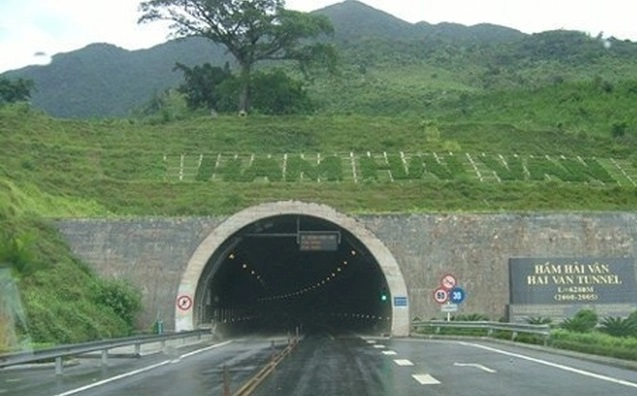
\includegraphics[width=.43\textwidth]{images/hamhaivan.jpg}};
	\begin{scope}[shift={(7,-1.3)}]
		\path (0,0) coordinate (O) (0:r) coordinate (A) (28:r) coordinate (B) 
		(2*28:r) coordinate (C) (3*28:r) coordinate (D) (3*28+12:r) coordinate (E) 
		(180:r) coordinate (H) (180-28:r) coordinate (G) (180-2*28:r) coordinate (F) 
		(180-3*28:r) coordinate (E) ($(H)!(F)!(A)$) coordinate (N) ($(H)!(C)!(A)$) coordinate (M)
		($(H)!(B)!(A)$) coordinate (K);
		\draw (H)--(A) (G)--(O)--(B) (F)--(O)--(C) (E)--(O)--(D) 
		(B)--node[scale=.8,sloped,above=-1pt]{$4{,}3$~m}(K) (A) arc (0:180:r);
		\draw  (0:.25) arc (0:84:.25) (96:.25) arc (96:180:.25);
		\foreach \i in {14,42,70,110,138,166}{\draw (\i:5pt)--++(\i:4pt);}
		\draw (M)--(N)--(F)--(C)--cycle;
		\draw[<->] (H)++(-90:.5)--++ (0:2*r)node[pos=.5,scale=.8,below]{$18$~m};
		\foreach \i/\j/\k in {C/M/O,B/K/O}{
			\draw ($(\j)!6pt!(\i)$)--($(\j)!6pt!(\k)-(\j)+(\j)!6pt!(\i)$)--($(\j)!6pt!(\k)$);};
		\foreach \i/\j in {O/-90,A/0,B/30,C/60,D/85,E/95,F/120,G/150,H/180,M/-90,N/-90,K/-90}
		\fill (\i) circle (1.2pt) node[shift={(\j:2.5mm)}]{$\i$};
	\end{scope}
	\end{tikzpicture}
\end{center}
\shortans{$7{,}6$}
\loigiai{
	Ta có: $OA=OB=\dfrac{18}{2}=9$ m.\\
	Xét tam giác $OBK$ vuông tại $K$, có:\\
	$\sin\widehat{BOK}=\dfrac{BK}{OB}=\dfrac{4{,}3}{9}\Rightarrow \cos\widehat{BOK}=\sqrt{1-{{\left(\dfrac{4{,}3}{9}\right)}^2}}\approx 0{,}88$.\\
	Xét tam giác $OCM$ vuông tại $M$, có:\\
	$\sin\widehat{COM}=\dfrac{CM}{OC}\Leftrightarrow CM=OC\cdot \sin\widehat{COM}=OC\cdot \sin\left(2\widehat{BOK}\right)$.\\
	$\sin\left(2\widehat{BOK}\right)=2\sin\widehat{BOK}\cdot \cos\widehat{BOK}\approx 2\cdot \dfrac{4\cdot3}{9}\cdot 0{,}88=\dfrac{946}{1125}$.\\
	Suy ra: $CM=9\cdot\dfrac{946}{1125}=\dfrac{946}{125}\approx 7{,}6$ m.\\
	Vậy chiều cao $CM$ cho phép của các xe lưu thông là $7{,}6$ m.}
\end{ex}

%%==========Câu 16

\TL{\textbf{\textit{(2,0 điểm)}}}
\begin{ex}%[1D1H3-4]
Rút gọn biểu thức $P = \dfrac{\cos a + 2\cos 3a + \cos 5a}{\sin a + 2\sin 3a + \sin 5a}$.
% \choice
% {$P = \tan a$}
% {$P = \cot a$}
% {\True $P = \cot 3a$}
% {$P = \tan 3a$}
\loigiai{
	Ta có: 
	$ \begin{aligned}[t] 
		P&=\dfrac{\cos a+2\cos 3a+\cos 5a}{\sin a+2\sin 3a+\sin 5a}=\dfrac{(\cos 5a+\cos a)+2\cos 3a}{(\sin 5a+\sin a)+2\sin 3a} \\
		&= \dfrac{2\cos 3a\cdot\cos 2a+2\cos 3a}{2\sin 3a\cos 2a+2\sin 3a}=\dfrac{2\cos 3a(1+\cos 2a)}{2\sin 3a(1+\cos 2a)}\\
		&= \dfrac{\cos 3a}{\sin 3a}=\cot 3a.
	\end{aligned}$
}
\end{ex}
%%==========Câu 17
% \begin{ex}%[1D1V3-5]
% Tìm giá trị lớn nhất $M$ của biểu thức $P=4{\sin ^2}x+\sqrt{2}\sin \left(2x+\dfrac{\pi }{4}\right)$ (làm tròn đến một chữ số thập phân).
% \shortans{$3{,}4$}
% \loigiai{
% 	Ta có:
% 	$ \begin{aligned}[t] 
% 		P &=4{\sin ^2}x+\sqrt{2}\sin \left(2x+\dfrac{\pi }{4}\right)=4\left(\dfrac{1-\cos 2x}{2}\right)+\sin 2x+\cos 2x \\
% 		&= \sin 2x-\cos 2x+2=\sqrt{2}\cdot\left(\dfrac{\sqrt{2}}{2}\sin 2x-\dfrac{\sqrt{2}}{2}\cos 2x\right)+2\\
% 		&= \sqrt{2}\left(\sin 2x\cdot\cos \dfrac{\pi }{4}-\cos 2x\cdot\sin \dfrac{\pi }{4}\right)+2=\sqrt{2}\sin \left(2x-\dfrac{\pi }{4}\right)+2.
% 	\end{aligned}$\\
% 	Mà $-1 \leq \sin \left(2 x-\dfrac{\pi}{4}\right) \leq 1 \Rightarrow-\sqrt{2}+2 \leq \sqrt{2} \sin \left(2 x-\dfrac{\pi}{4}\right)+2 \leq \sqrt{2}+2$.\\
% 	Vậy giá trị lớn nhất của $P$ là $3{,}4$.}
% \end{ex}

%%==========Câu 18
% \begin{ex}%[1D1V3-7]
% \immini{
% Một sợi cáp $R$ được gắn vào một cột thẳng đứng ở vị trí cách mặt đất $14$ m. Một sợi cáp $S$ khác cũng được gắn vào cột đó ở vị trí cách mặt đất $12$ m. Biết rằng hai sợi cáp trên cùng được gắn với mặt đất tại một vị trí cách chân cột $15$ m (hình vẽ).Tính $\tan \alpha$, ở đó $\alpha $ là góc giữa hai sợi cáp trên (làm tròn đến một chữ số thập phân).
% }{
% \begin{tikzpicture}[scale=.8,font=\footnotesize,>=stealth]
% 	\path (0,0) coordinate (H) (0,3) coordinate (B) (0,4) coordinate (A) (4,0) coordinate (O) (1,.5) coordinate (H') (1,3.5) coordinate (B') (1,4.5) coordinate (A')
% 	(H)++(180:.6) coordinate (H'')++(180:.6) coordinate (H''')
% 	(B)++(180:.6) coordinate (B'') (A)++(180:1.2) coordinate (A'');
% 	\draw pic["$\beta$"{scale=.8},draw, angle radius = 15pt,angle eccentricity=1.3]{angle = A--O--H};
% 	\draw pic[draw,double, angle radius = 25pt,angle eccentricity=1.6]{angle = A--O--B};
% 	\draw[->] (O)++(140:1)--++(0:.7)node[right]{$\alpha$};
% 	\draw (A)--(O)--node[below,scale=.8]{$15$~m}(H) (O)--(B) (H)--(H') (B)--(B') (A)--(A');
% 	\draw[ultra thick] (A)--(H) (A')--(H');
% 	\draw[dashed] (H)--(H''') (B)--(B'') (A)--(A'');
% 	\draw[<->] (H'')--node[fill=white,scale=.8]{$12$~m}(B'');
% 	\draw[<->] (H''')--node[pos=.6,fill=white,scale=.8]{$14$~m}(A'');
% 	\foreach \i/\j in {A/100,B/140,O/-60,H/-90}
% 	\fill (\i) circle (1.2pt) node[shift={(\j:2.5mm)}]{$\i$};
% \end{tikzpicture}
% }

% \shortans{$0{,}1$}
% \loigiai{
% 	Xét $\triangle AOH$ vuông tại $H$, ta có: $\tan\beta =\dfrac{AH}{HO}=\dfrac{14}{15}$.\\
% 	Đặt $\widehat{BOH}=\gamma$.\\
% 	Xét $\triangle BOH$ vuông tại $H$, ta có: $\tan\gamma =\dfrac{BH}{HO}=\dfrac{12}{15}=\dfrac{4}{5}$.\\
% 	$\tan\alpha =\tan\left(\beta -\widehat{BOH}\right)=\tan(\beta -\gamma)=\dfrac{\tan\beta -\tan\gamma }{1+\tan\beta \tan\gamma }=\dfrac{\dfrac{14}{15}-\dfrac{4}{5}}{1+\dfrac{14}{15}\cdot \dfrac{4}{5}}=\dfrac{\dfrac{2}{15}}{\dfrac{131}{75}}=\dfrac{10}{131}$.\\
% 	Vậy $\tan\alpha \approx 0{,}1$.
% }
% \end{ex}
\Closesolutionfile{ans}
% \indapan{6}{ans/ans-1-B2-3}
